
\section{Experiment}
\subsection{Phase 1.1 - Frozen Training}

Each network was trained ten times over the course of three hours resulting in a representatively distributed set of trained networks.
Figure \ref{fig:frozen_training_times} visualizes the relations between the average training times.

\begin{tikzpicture}
\begin{axis}[
    ybar,
    width=0.8\linewidth, height=50mm,
    ymax=270,
    ytick=\empty,
    bar width=2mm,
    ymajorgrids,
    ylabel={Average Training Time (s)},
    extra y ticks={30, 60, 90, 120, 180, 240},    
    xtick=data,
    symbolic x coords={EfficientNetB0, InceptionResNetV2, MobileNet, NASNetLarge, ResNet50V2, VGG16, Xception},
    nodes near coords,
    nodes near coords style={/pgf/number format/.cd,precision=0},
    x tick label style={rotate=-45,anchor=west}
    ]
    \addplot table [y={avgtme}]{\frozentrainingtable};
\end{axis}
\end{tikzpicture}

No linear relation between parameter count and training time can be determined.
NasNetLarge takes by far the longest to train with an average of approximately 3.5 minutes. 
MobileNet was the fastest to train with slightly under 30 seconds.


\begin{tikzpicture}
\begin{axis}[
    ymode=log,
    width=0.7\linewidth, height=50mm,
    log basis y=10,
    grid=major,
    boxplot/draw direction=y,
    scale only axis,            
    legend style={
        at={(1.00,0.5)},
        anchor=west},
    ytick=\empty,
    ymax=1,
    ylabel={Validation Accuracy},
    extra y ticks={0.25, 0.5, 0.6, 0.7, 0.8, 0.9},
    extra y tick labels={25\%, 50\%, 60\%, 70\%, 80\%, 90\%},
    xtick=\empty,
    extra x ticks={1, 2, 3, 4, 5, 6, 7, 8, 9, 10, 11},
    extra x tick labels={efficientnet, inceptionresnetv2, mobilenet, mobilenetv2, mobilenetv3, nasnetlarge, nasnetmobile, resnetv2, vgg16, vgg19, xception},
    extra x tick style={
        grid=major,
        tick label style={rotate=-45,anchor=west}}]

        \pgfplotstablegetrowsof{\frozentrainingtable}
        \pgfmathtruncatemacro\TotalRows{\pgfplotsretval-1}
        \pgfplotsinvokeforeach{0,...,\TotalRows}{
            \addplot+[
            boxplot prepared from table={
                table=\frozentrainingtable,
                row=#1,
                lower whisker=min_acc,
                upper whisker=max_acc,
                average=avg_acc
            },
            boxplot prepared,
                % to get a more useful legend
                area legend
            ]
            coordinates {};
        }
\end{axis}
\end{tikzpicture}



Many networks hover around 90\% validation accuracy for their best case.
The earliest insight is that light-weight, small networks are up to par with bigger, much more complex implementations in the context of this experiment.
An additional number of parameters does not seem to indicate better prediction accuracy for binary classifications.
Even smaller networks obtain the same or a better average validation accuracy.

InceptionResnetV2 has a high accuracy fluctuation between training sessions which could not be attributed to any superficial property and the reason behind it is unclear.
On average, the aforementioned network performed the worst while being the second largest.

After the training phase, the best-case networks were identified using the average validation accuracy.
The weights for each node are persisted and can be downloaded and applied to reproduce the predictions.
The following analysis will feature these persisted models.


\subsection{Phase 1.2 - Liquid Training}
All networks are trained again with the same configuration, but now all layers are able to adapt their parameters.
Immediately noticeable is the drastic increase in training time for each network.
Another important fact is the increase in resource consumption of unfrozen layers during the training phase.
The training was terminating multiple times during training iterations with variations of out-of-memory exceptions.
Figure \ref{fig:liquid_training_times} visualizes the relations between the average training times once again.


\begin{tikzpicture}
\begin{axis}[
    ybar,
    width=0.8\linewidth, height=50mm,
    ymin=0,ymax=2640,
    ytick=\empty,
    bar width=2mm,
    ymajorgrids,
    ylabel={Average Training Time (s)},
    extra y ticks={300, 600, 1200, 1800, 2400},
    extra y tick labels={5min, 10min, 20min, 30min, 40min},
    xtick=data,
    symbolic x coords={efficientnet, inceptionresnetv2, mobilenet, mobilenetv2, mobilenetv3, nasnetlarge, nasnetmobile, resnetv2, vgg16, vgg19, xception},
    nodes near coords,
    nodes near coords style={/pgf/number format/.cd,precision=0},
    x tick label style={rotate=-45,anchor=west}
    ]
    \addplot table [y={avg_tme}]{\liquidtrainingtable};
\end{axis}
\end{tikzpicture}


NasNetLarges training time increased tenfold and it takes almost 40 minutes on average.


\begin{tikzpicture}
\begin{axis}[
    ymode=log,
    width=0.7\linewidth, height=40mm,
    log basis y=10,
    grid=major,
    boxplot/draw direction=y,
    scale only axis,            
    legend style={
        at={(1.00,0.5)},
        anchor=west},
    ytick=\empty,
    ymax=100,
    ylabel={Validation Accuracy},
    extra y ticks={25, 50, 60, 70, 80, 90},
    extra y tick labels={25\%, 50\%, 60\%, 70\%, 80\%, 90\%},
    xtick=\empty,
    extra x ticks={1, 2, 3, 4, 5, 6, 7, 8, 9, 10, 11},
    extra x tick labels={EfficientNetB0, InceptionResNetV2, MobileNet, NASNetLarge, ResNet50V2, VGG16, 
Xception},
    extra x tick style={
        grid=major,
        tick label style={rotate=-45,anchor=west}}]

        \pgfplotstablegetrowsof{\liquidtrainingtable}
        \pgfmathtruncatemacro\TotalRows{\pgfplotsretval-1}
        \pgfplotsinvokeforeach{0,...,\TotalRows}{
            \addplot+[
            boxplot prepared from table={
                table=\liquidtrainingtable,
                row=#1,
                lower whisker=minacc,
                upper whisker=maxacc,
                average=avgacc
            },
            boxplot prepared,
                % to get a more useful legend
                area legend
            ]
            coordinates {};
        }
\end{axis}
\end{tikzpicture}



The increased time spent for a more thorough training phase was worth it as almost all networks now break the 90\% validation accuracy barrier.
InceptionResnetV2 delivers a respectable top accuracy after the disappointing result in the last section.


\begin{table}[htb]
\centering

    \begin{tabular}{ l  r  r  r } \hline
    Network Name       & frozen & delta    & liquid \\ \hline 
    efficientnet       & 90.29  &  +3.0\%  & 93.10 \\
    inceptionresnetv2  & 66.39  & +29.6\%  & 94.33 \\
    mobilenet          & 89.63  &  +2.0\%  & 91.44 \\
    nasnetlarge        & 78.88  & +12.4\%  & 90.05 \\
    resnetv2           & 84.41  &  +7.2\%  & 90.99 \\
    vgg16              & 89.47  &  -2.2\%  & 87.57 \\
    xception           & 78.58  & +17.6\%  & 95.32 \\ \hline 
    \end{tabular}

    \caption{Difference in Top Validation Accuracy}
    \label{tbl:training_diff}
\end{table}


Table \ref{tbl:training_diff} shows the relative gain in validation accuracy of frozen versus freely trained networks.
Many of the smaller networks do not gain much, but on the other hand, InceptionResnetV2 and Xception are now much more competitive.
Xceptions best validation accuracy is comparabale with some of the algorithms handed in during the LivDet2017 competition in regards to the dataset this experiment uses. \cite{LIVDET}

\hfill

\subsection{Phase 2 - Prediction Analysis}
Serialized models are loaded and the testing dataset will be interpreted once again while capturing confidence values for further analysis.
The detection error trade-off curve confirms that none of the networks have a clear advantage compared to each other, but shows that NasNet Large and NasNet Mobile performed the worst with an average difference of TBD \% and TBD \% respectively.



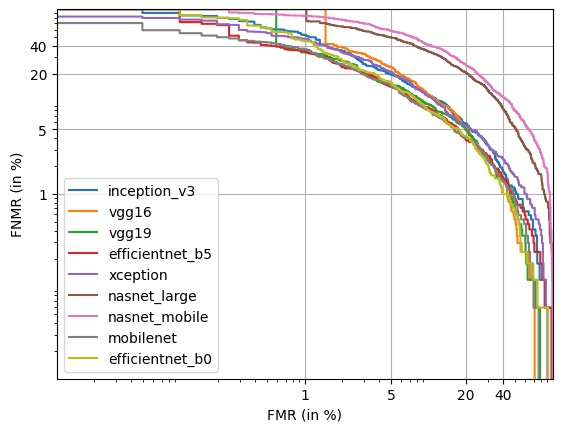
\includegraphics[width=\linewidth]{det-all.jpg}


In the following subsections, each network will be inspected individually by evaluating the performance implicitly assuming a neutral FNMR and FMR rate balancing false positives and false negatives.
This allows the performance to be differentiated in terms of certain materials.


\newpage
\subsubsection{EfficientNet B0}
Even before unfreezing all layers EfficientNetB0 was providing a usable PAD detection accuracy.
Only a small increase in accuracy could be gained by liquid training.
Interestingly, the correct non-match rate increased by almost 6\% while the correct match rate sank slightly.

Prediction latencies are consistent, but the few outliers make the average time quite a lot higher than the median latency as seen in Table \ref{tbl:efficientnet_latencies}.

\predictiontables{EfficientNetB0}


\subsubsection{Inception Resnet V2}
A surprising increase in prediction accuracy of almost 30\% was observed for InceptionResnetV2.
The detection scores for all materials benefitted from the liquid training.
Liquid Ecoflex was already reliably detected by the network but is now detected more reliably.
The network gained significant detection capabilities for all other materials.

An average latency of 60ms is slow compared to the other networks.

\predictiontables{InceptionResNetV2}


\subsubsection{MobileNet}
Not a lot improved for MobileNet by unfreezing the layers and in case of Gelatine some accuracy was lost.
Bona fide fingerprints were correctly detected with an accuracy of 91.7\% and 94.4\%, while attack presentations were detected correctly with 87.9 and 89.0\%.

With the relatively inaccurate detection comes the shortest latency with an average of 27ms.
MobileNet was the fastest network in this experiment to deliver a prediction result.

\predictiontables{MobileNet}


\subsubsection{Nasnet Large}
Liquid Ecoflex samples were correctly classified most of the time with a high average rate of 99.7\% after the unfrozen training.
The high attack presentation detection is unfortunately paired with a low correct match rate of only 80\% after unfrozen training, which is the lowest in the entire experiment.

With an average of almost 73ms NasNetLarge has the highest prediction latency.

\predictiontables{NASNetLarge}


\subsubsection{Resnet V2}
Liquid Ecoflex samples were again correctly classified most of the time with a similar rate of 99.1\% after liquid training.
BPCER and APCER are more balanced and result in an overall better accuracy in comparison to NasNetLarge.
The average prediction latency is half of NasNetLarges.

\predictiontables{ResNet50V2}


\subsubsection{VGG16}
The liquid training resulted in a drastic decrease of bona fide fingerpint recognition and compared to that only a minor increase in correct non-match rate was gained.
VGG16 is the only network that lost accuracy after liquid training.

\predictiontables{VGG16}


\subsubsection{Xception}
The best performer in the test has a correct non-match rate of 97.5\% and returns a prediction result in under 36ms, which is quite fast in comparison to the other networks.
Presentation attacks were able to be detected precisely with a max delta of under 1\%.

\predictiontables{Xception}




\endinput





\subsubsection{EfficientNet B0}

The only BPCER over 90\% is achieved by EfficientNet B0 which is the second best performer over all.
Bona fide fingerprints were correctly detected with an accuracy of 92.5\%.

\predictiontables{efficientnet}



\medskip
Out of the three tested neural networks MobileNet was performing the best on average thanks to it's high true negative detection rate.
The other two networks however have a better true positive rate.
\bigskip\hrule



\subsection{MobileNet}
Bona fide fingerprints were correctly detected with an accuracy of 89.1\%, while presentation attacks were detected correctly with 93.19\%.
None of the materials show significant variance from each other and are within a range of 92.0\% and 94.7\%.
Liquid Ecoflex shows the worst deception potential.


\predictiontables{mobilenet}




\subsection{Nasnet Mobile}

With a CMR of 81.2\% Nasnet Mobile is the worst performer in the small network group.
The presentation attack detection for the Latex datasets was with only 63\% slightly better than randomly assigned outcomes.
A low precision in regards to the materials provide an interesting difference of over 20\% accuracy between Latex and Liquid Ecoflex.



\medskip
Out of the three tested neural networks MobileNet was performing the best on average thanks to it's high true negative detection rate.
The other two networks however have a better true positive rate.
\bigskip\hrule



\subsection{Xception}
    Presentation attack were able to be detected precicely with a max delta of 2.9\% and all accuracies are over 90\%.
    The overall performance is nothing outstanding and is in line with the median.




\subsection{Inception V3}

    The performance is very similar to the previous network with the accuracies differing by only 0.08\%.
    Inception V3s bona fide detection is a little better, but in turn resentation attacks a bit worse in comparison.




\subsection{EfficientNet B5}

    The highest correct non-match rate in the entire series is held by EfficientNet B5 with 96.03\% which is up to par with specialized solutions (cite livdet2017, p7).
    EfficientNet B5 is the best performer on average in the medium size category but the other two networks are very close in accuracy.

Networks in the midrange size deliver as strong performance and are precise in their accuracies.
EfficientNet B5 has the second best accuracy as well as the best APCER.

\bigskip\hrule


\subsection{NASNet Large}
\begin{minipage}[c]{0.7\textwidth}
    More than a fifth of all predictions were incorrect which makes NASNet Large not suitable to enhance the quality of fingerprint presentation attack detection mechanisms.
    With almost 18.2\% of difference between Latex and Liquid Ecoflex, the precision is the worst among all tested networks.

    \medskip\centering Match Rates: 
    \begin{tabular}{ r  r  r  r |}
        BPCER       & APCER      & FNMR     & FMR     \\
        80.11\%   & 79.41\%   & 20.59\%  & 19.89\%  \\
    \end{tabular} \hspace{2mm} Accuracy: 79.73\%
\end{minipage}
\hfill
\begin{minipage}[t]{0.3\textwidth}
    \centering
    
\begin{tabular}{ c   r }
    Live               &  80.1\% \\ \hline\hline
    Latex\_02           & 70.6\% \\
    Latex\_01           & 71.2\% \\
    Gelatine\_02        & 77.1\% \\
    Gelatine\_01        & 80.9\% \\
    Liquid\_Ecoflex\_02 & 87.9\% \\
    Liquid\_Ecoflex\_01 & 88.8\%
\end{tabular}
\end{minipage}



\subsection{VGG16}
\begin{minipage}[c]{0.7\textwidth}
    The second largest network in this test did not deliver any outstanding data.
    Accuracy and precision are certainly respectable and in the better half of all tested networks, but unremarkable considering the size and prediction latency.

    \medskip\centering Match Rates: 
    \begin{tabular}{ r  r  r  r |}
        BPCER       & APCER      & FNMR     & FMR     \\
        87.88\%   & 90.29\%   & 9.71\%   & 12.12\%  \\
    \end{tabular} \hspace{2mm} Accuracy: 89.19\%
\end{minipage}
\hfill
\begin{minipage}[c]{0.3\textwidth}
    \centering
    \begin{tabular}{ c   r }
    Live                & 87.9\% \\ \hline\hline
    Latex\_02           & 86.8\% \\    
    Liquid\_Ecoflex\_02 & 88.5\% \\
    Liquid\_Ecoflex\_01 & 89.7\% \\
    Latex\_01           & 91.5\% \\
    Gelatine\_02        & 92.4\% \\
    Gelatine\_01        & 92.9\% \\
\end{tabular}

\end{minipage}



\subsection{VGG19}
\begin{minipage}[c]{0.7\textwidth}
    The largest network provides solid non-match recognition, but cannot provice a good accuracy.
    A APCER of almost 94\% is the second highest score comparable to algorithms which were handed in for LivDet2017.

    \medskip\centering Match Rates: 
    \begin{tabular}{ r  r  r  r |}
        BPCER       & APCER      & FNMR     & FMR     \\
        86.93\%   & 93.38\%   & 6.62\%   & 13.07\%  \\
    \end{tabular} \hspace{2mm} Accuracy: 90.45\%
\end{minipage}
\hfill
\begin{minipage}[c]{0.3\textwidth}
    \centering
    \begin{tabular}{ c   r }
    Live                & 86.9\% \\ \hline\hline
    Latex\_02           & 90.6\% \\ 
    Liquid\_Ecoflex\_01 & 92.4\% \\
    Liquid\_Ecoflex\_02 & 93.2\% \\
    Latex\_01           & 93.8\% \\
    Gelatine\_02        & 94.7\% \\
    Gelatine\_01        & 95.6\%
\end{tabular}

\end{minipage}


Especially with regards to NASNet Large, the additional size seems to provide no benefit to fingerprint presentation attack-detection mechanisms.
For NASNet Large in particular, the additional size does not provide any benefit to fingerprint presentation attack-detection mechanisms.
VGG16 and VGG18 ware both marginally better than the average network and did not deliver the expected accuracy or precision.
